%% bare_jrnl.tex
%% V1.4b
%% 2015/08/26
%% by Michael Shell
%% see http://www.michaelshell.org/
%% for current contact information.
%%
%% This is a skeleton file demonstrating the use of IEEEtran.cls
%% (requires IEEEtran.cls version 1.8b or later) with an IEEE
%% journal paper.
%%
%% Support sites:
%% http://www.michaelshell.org/tex/ieeetran/
%% http://www.ctan.org/pkg/ieeetran
%% and
%% http://www.ieee.org/

%%*************************************************************************
%% Legal Notice:
%% This code is offered as-is without any warranty either expressed or
%% implied; without even the implied warranty of MERCHANTABILITY or
%% FITNESS FOR A PARTICULAR PURPOSE! 
%% User assumes all risk.
%% In no event shall the IEEE or any contributor to this code be liable for
%% any damages or losses, including, but not limited to, incidental,
%% consequential, or any other damages, resulting from the use or misuse
%% of any information contained here.
%%
%% All comments are the opinions of their respective authors and are not
%% necessarily endorsed by the IEEE.
%%
%% This work is distributed under the LaTeX Project Public License (LPPL)
%% ( http://www.latex-project.org/ ) version 1.3, and may be freely used,
%% distributed and modified. A copy of the LPPL, version 1.3, is included
%% in the base LaTeX documentation of all distributions of LaTeX released
%% 2003/12/01 or later.
%% Retain all contribution notices and credits.
%% ** Modified files should be clearly indicated as such, including  **
%% ** renaming them and changing author support contact information. **
%%*************************************************************************


% *** Authors should verify (and, if needed, correct) their LaTeX system  ***
% *** with the testflow diagnostic prior to trusting their LaTeX platform ***
% *** with production work. The IEEE's font choices and paper sizes can   ***
% *** trigger bugs that do not appear when using other class files.       ***                          ***
% The testflow support page is at:
% http://www.michaelshell.org/tex/testflow/


% Please refer to your journal's instructions for other
% options that should be set.
\documentclass[journal,onecolumn,11pt]{IEEEtran}
%
% If IEEEtran.cls has not been installed into the LaTeX system files,
% manually specify the path to it like:
% \documentclass[journal]{../sty/IEEEtran}


\makeatletter
\def\endthebibliography{%
  \def\@noitemerr{\@latex@warning{Empty `thebibliography' environment}}%
  \endlist
}
\makeatother

\usepackage{graphicx}
\usepackage{hyperref}
\usepackage[skip=2pt,belowskip=-2pt,labelfont=bf,font=small]{caption}
\captionsetup[table]{name=Table}
\captionsetup[figure]{name=Figure}
\usepackage[margin=1in]{geometry}
\usepackage{times}
\usepackage{amsmath}
\usepackage{algpseudocode}
\usepackage{algorithm, algorithmicx}


\begin{document}
%
% paper title
% Titles are generally capitalized except for words such as a, an, and, as,
% at, but, by, for, in, nor, of, on, or, the, to and up, which are usually
% not capitalized unless they are the first or last word of the title.
% Linebreaks \\ can be used within to get better formatting as desired.
% Do not put math or special symbols in the title.
\title{Privacy-preserving, location-based queries using DHTs and R-Trees}
%
%
% author names and IEEE memberships
% note positions of commas and nonbreaking spaces ( ~ ) LaTeX will not break
% a structure at a ~ so this keeps an author's name from being broken across
% two lines.
% use \thanks{} to gain access to the first footnote area
% a separate \thanks must be used for each paragraph as LaTeX2e's \thanks
% was not built to handle multiple paragraphs
%

\author{Giovanni Campagna, Keshav Santhanam}

% make the title area
\maketitle

% As a general rule, do not put math, special symbols or citations
% in the abstract or keywords.
\begin{abstract}
Abstract goes here.
\end{abstract}

\section{Introduction}
Social running applications such as Strava~\cite{strava} provide an easy way for users to track their activity and share it with friends. However, these applications lack the ability to pair together runners who share similar routes. This task is not trivial as there are several constraints that must be met in order for such an application to be widely adopted:
\begin{itemize}
	\item Users of the application must be able to share their routes with other users
	\item The application should be able to compute similar routes quickly
	\item Users should not be able to see the exact location of any other user
\end{itemize}
To satisfy these constraints we present hDHT, a distributed system that combines the geo-distributed key-value lookup capabilities of a distributed hash table (DHT) with the fast, location-based queries enabled by Hilbert R-Trees~\cite{kamel1993hilbert}.
This paper proceeds as follows. Section~\ref{section:background} introduces the technologies of DHTs and Hilbert R-Trees. Section ~\ref{section:design} provides a high-level overview of our system architecture. Section~\ref{section:implementation} delves into the implementation details of hDHT. Section~\ref{section:evaluation} highlights some experimental results based on microbenchmarks [TODO: decide if is this necessary]. Section~\ref{section:related-work} discusses alternative approaches to this problem. Section~\ref{section:future-work} enumerates potential next steps for this project and Section~\ref{section:conclusion} concludes.
\section{Background} \label{section:background}
In this section we give a brief overview of the core technologies that support hDHT.

\subsection{Distributed hash tables}
A distributed hash table (DHT) is a decentralized system that supports efficient, distributed key-value lookups by maintaining a subset of the total keyspace on each node. Nodes forward requests for keys that are outside its own keyspace to other nodes in the system by keeping some information about its peers, each of which is responsible for a different segment of the keyspace. Early efforts to study DHTs include Chord~\cite{stoica2001chord}, Tapestry~\cite{zhao2001tapestry}, and Pastry~\cite{rowstron2001pastry}.

\subsection{Hilbert R-Trees}
Kamel and Faloutsos proposed the idea of a Hilbert R-Tree as a means of performing efficient location-based queries~\cite{kamel1993hilbert}. Their key insight was that by using a Hilbert curve to determine a linear ordering of the entries in the tree, the splitting policy in overflow scenarios can be tuned in such a way that the utilization of the tree is close to 100\%. Each node in a Hilbert R-Tree keeps track of the largest Hilbert value (LHV) among the entries in its subtree, as well as the maximum bounding rectangle (MBR) over all its subtree entries. Entries are then inserted in order of increasing Hilbert value, and the LHV and MBR of each node are adjusted as necessary after every modification to the tree.
\section{System Design} \label{section:design}

The goal of our system is to store the location, and associated information, of a large number of clients who can potentially move around in the real world.
Once the location is stored, our system can serve requests against those clients efficiently, leveraging the physical locality properties.
In this section, we introduce the design, while Section~\ref{section:implementation} discusses some tradeoffs in our implementation.

\subsection{Architecture}

\begin{figure}
\centering
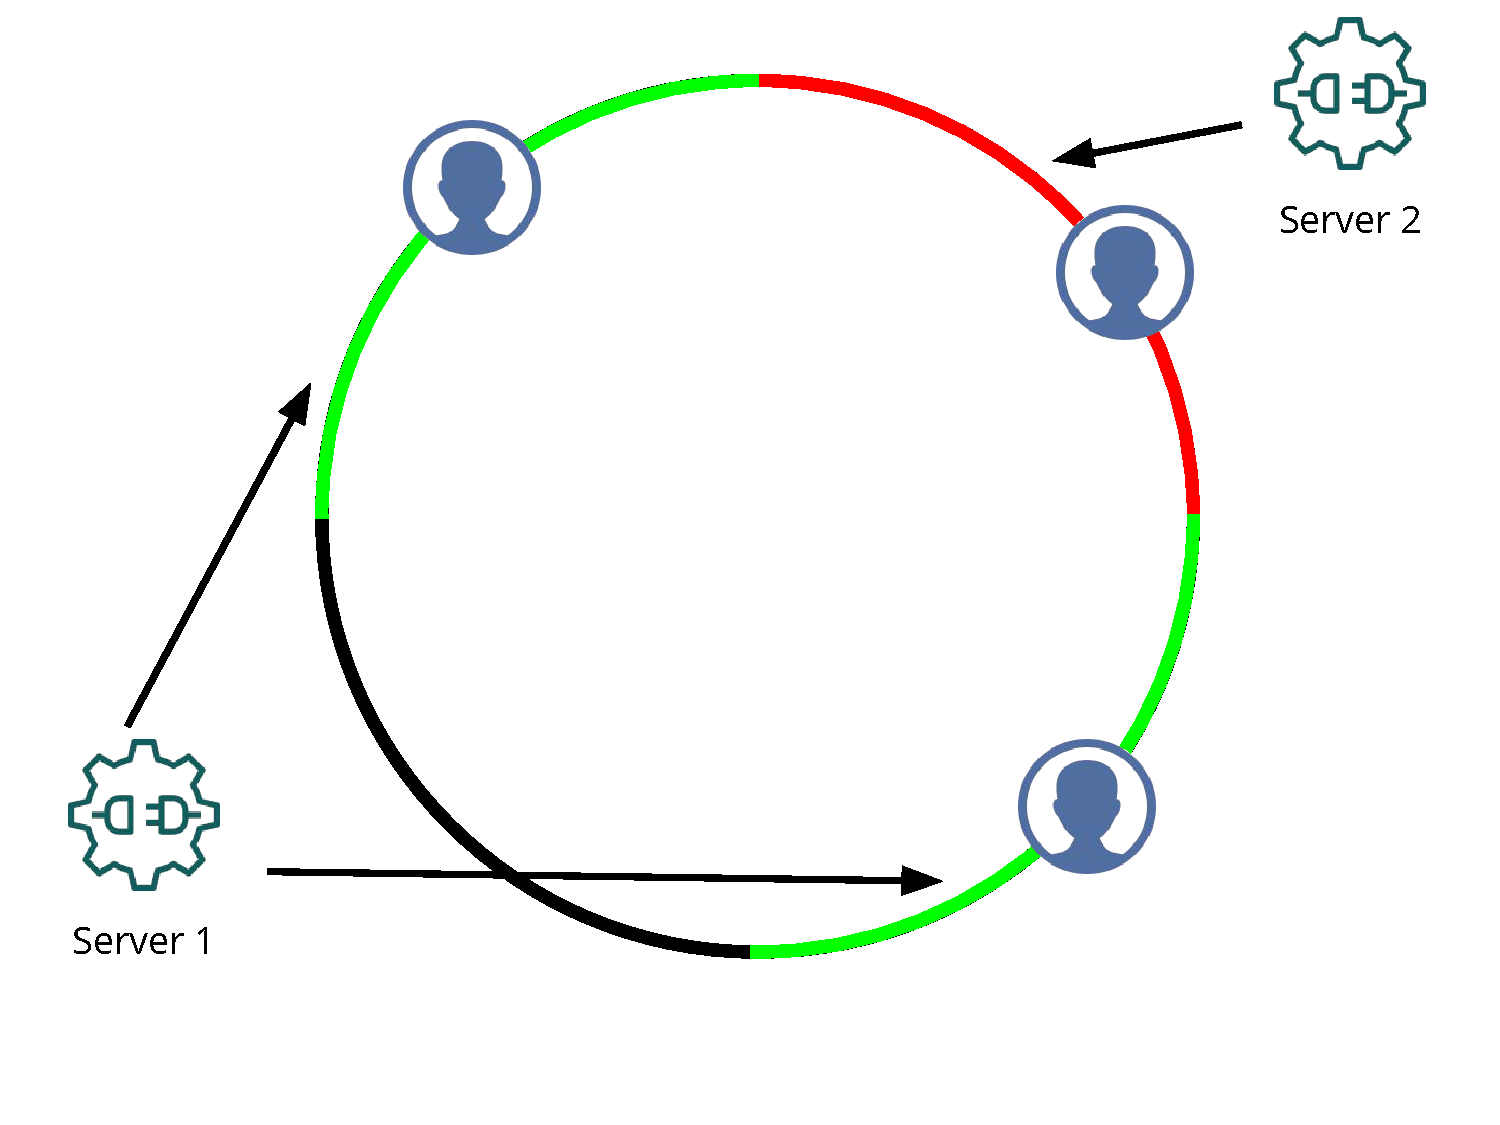
\includegraphics[width=0.6\linewidth]{figures/arch.pdf}
\caption{The Architecture of hDHT.}
\label{fig:arch}
\end{figure}

The architecture of hDHT is shown in Figure~\ref{fig:arch}.
In hDHT, the server control one or more contiguous segments on a \textit{consistent hashing ring}~\cite{}.
Each client has a position in the hashing ring which is determined based on the client physical location, using the \textit{Hilbert curve function}~\cite{}.
Each client thus \textit{registers} with the server that controls the segment containing the client.

In the example, Server 1 controls the two green segments, and stores the data for two clients.
Server 2 controls the red segment, and stores the data only of the client in that segment.
Other servers, not shown, control the rest the DHT curve.

\subsection{Client Interface}

Clients of hDHT are likely to be on a mobile device, as they should follow and record precisely the location of the user.
Servers cannot perform RPCs towards the clients, because the clients might be behind a restrictive firewall.
For this reason, our design moves most of the computation and networking to the server, and initiates all client-server communication from the client.

Each client is identified by a 160-bit node identifier.
This identifier is opaque to the client.
The client additionally stores its own position, as obtained from the GPS senstor, and the address of the server it is registered with.
The client interacts primarily with the registering server, but any time it can retrieve the address of the server responsible for any point in the curve.

Servers store simple client metadata, in the form of string key-value pairs.
Each server serves metadata requests only for the clients it is responsible for, which ensures consistency.

The full client-server interface is shown in Figure~\ref{fig:client-server}.

\begin{figure}
\small
\begin{itemize}
\item $\textsc{FindControllingServer}(\textit{node\_id}) \rightarrow \textit{address}$: find the address of the server controlling the given node ID; this request succeeds even if the node ID does not correspond to any client registered with the server
\item $\textsc{FindServerForPoint}(\textit{position}) \rightarrow \textit{address}$: find the address of the server controlling the given position
\item $\textsc{ClientHello}(\textit{position}, \textit{node\_id}) \rightarrow \textit{ok}, \textit{node\_id}$: register the client against this server; the client transmits both its own position and the previously obtained node ID, if available; the server responds \textit{Created} if the client was newly registered, \textit{AlreadyExists} if it recognized the previous node ID, or \textit{WrongServer} if the server is not responsible for the region of the Hilbert curve corresponding to \textit{position}.
\item $\textsc{Move}(\textit{position}) \rightarrow \textit{ok}, \textit{node\_id}, \textit{address}$: informs the server that the client moved; the server replies with the new node ID for the client, and either \textit{SameServer} or \textit{DifferentServer}, to indicate what server is now responsible for the client; if the client receives \textit{DifferentServer}, it must register with the new server
\item $\textsc{SetMetadata}(\textit{key}, \textit{value})$: set metadata for the calling client
\item $\textsc{GetMetadata}(\textit{node\_id}, \textit{key}) \rightarrow \textit{value}$: get metadata about the given client; the server forwards the request to the controlling server if needed
\end{itemize}
\caption{The hDHT client-server protocol}
\label{fig:client-server}
\end{figure}

\subsection{Hilbert Curves}

Client node IDs define the position of a client in the consistent hashing ring.
To facilitate location based queries, the node IDs are generated using a \textit{locality sensitive hash} that uses a Hilbert curve.

A Hilbert curve, or \textit{space-filling curve}, is a curve that passes all points in a grid exactly once and does not self intersect.
Hilbert curve can be constructed for grids of arbitrary dimension.
The Hilbert curve of order $k$, which covers the grid of size $2^k \times 2^k$, is constructed as a fractal, by refining the Hilbert curve of order $k-1$.
An efficient $O(k)$ algorithm exists to convert any point to the Hilbert curve to its coordinates in the grid and viceversa.

\subsection{Mapping Hilbert Curves to Consistent Hashing}

hDHT uses the Hilbert curve concept to generate the ID of the client.
First, the physical position of the client is mapped to a point in a rectangular Earth-sized grid.
Then, the point in the grid is converted to a point in the Hilbert curve, which provides the high bits of the node IDs.
The remaining low bits are assigned randomly.
This is a locality sensitive hashing because clients who are phyisically close will have similar Hilbert curve values, and thus will share some of the high bits of their node IDs.
Additionally, clients with similar high bits in the node IDs are more likely to be assigned to the same server, which improves the efficiency of serving requests.

Furthermore, hDHT must partition the grid in a way that each server controls a rectangular region.
This way, search requests can be served efficiently by dividing the query into disjoint rectangles.
To do so, the Hilbert curve must be partitioned into \textit{intervals} of the form:
\begin{align}
\left[k 2^i, (k+1) 2^i\right)
\end{align}
(with $k$, $i$ integers, and $i$ less than the order of the curve).
Intervals of this form can be shown to be non-overlapping in the grid.

Each server controls one or more of these intervals.
The server has complete information over the intervals it controls, and relies on other servers for the rest of the grid.


\subsection{Search Inside a Single Interval}
For each controlled interval of the Hilbert curve, the server maintains an \textit{Hilbert RTree}~\cite{} of the clients.
This is a data structure that allows efficient insertion, deletion and query by rectangle.

FINISHME...

\subsection{Search Across the Whole Space}
To perform a search, the server needs to efficiently identify which intervals of the DHT are partially covered by the search rectangle, and then perform the search within the interval.

The takes advantage of an important property of Hilbert curves: if a point is outside a rectangle in the Hilbert curve, all points on the curve between that point and the next rectangle corner are also outside the corner.

The server then uses the following algorithm:
\begin{enumerate}
\item First it computes the Hilbert values $h_0, h_1, h_2, h_3$ of the four corners of the rectangle, where $h_0$ is the smallest Hilbert value and $h_3$ is the largest
\item The algorithm keeps track of a \textit{current point}, initialized to $h_0$.
\item Then, it checks if the current point is inside the query rectangle.
\item If so, it finds the interval that contains the current point from the DHT
\item For a local interval, it uses the RTree to perform the search
\item For a remote interval, it forwards the search to the server that controls the interval, and merges the result
\item The algorithm then proceeds at point $h'$ immediately after the end of the interval in the Hilbert curve $h' = (k+1) 2^i$
\item If the current point is outside the query rectangle, the algorithm sets to current point to the minimum of $h_i$ that is strictly greater than the current point (in other words, it skips to the next corner of the query rectangle in the Hilbert curve).
\item The algorithm terminates when the current point is greater than $h_3$.
\end{enumerate}

\subsection{Routing and Load Balancing}

To make it possible for servers to join and leave the DHT easily, each server does not keep precise information on which intervals are owned by whom.

At initialization time, the server starts with a single peer, which it assumes controls the whole table.
The server registers with this initial peer, who responds with a list of interval it knows about.
The server then registers with each of the newly discovered peers, which will further send more and more precise information.

Additionally, when a new server joins the DHT, each peers that learns about the new server performs load balancing on the portion of the table it controls, by spilling the intervals it controls and transferring control of the newly created subintervals to the new server.
Intervals must be split in half at each step, because they must be power-of-2 sized to be rectangular in the grid.

An interval will be considered for splitting if it is larger than a threshold (in logarithmic size), or if the number of clients exceeds a threshold.
In the former case, the interval is split in half only once, and one half is sent to the new server.
In the latter case, the newly created half interval with the most clients is split again until the number of clients is below the threshold.
Then, the half interval with the least clients is sent to the new server.

Servers automatically move the metadata and client IDs during DHT rebalancing, but they do not inform clients.
Clients learn of the rebalancing by receiving a redirection error the next time they attempt to perform a request.

\section{Implementation} \label{section:implementation}

hDHT was implemented as a self contained library, as well as a daemon to act as the server.
The hDHT library also includes an example command line client, which allows one to test the capabilities of the system without physically moving around.

hDHT is open source, and available on Github~\footnote{\url{https://github.com/gcampax/hDHT}}. We implemented hDHT in approximately 5,000 lines of C++ code.

\subsection{Library Design}

hDHT uses C++, and the libuv library~\footnote{\url{http://libuv.org}} for the event loop and asynchronous portable IO.
It has been tested on Linux and OS X.

The client API of the library consists of a single \texttt{Client} object, which exposes methods to get and set the current location, get and set the local metadata, and perform queries against remote clients.
All other objects in the library, including the R-Tree implementation and the DHT abstraction, are hidden from library users.

To aid in code reuse, and reduce disk footprint, the library also includes the full server implementation. The server binary is a shim that initializes the library in server mode.

\subsection{R-Tree}
We built a self-contained R-Tree library from scratch by using the algorithms provided in the Hilbert R-Tree paper~\cite{kamel1993hilbert}. The \texttt{RTree} class provides a minimal interface to allow for inserting data
into the tree at a particular \texttt{Point} in the 2D space and performing a search using a \texttt{Rectangle}. The search returns a list of \texttt{NodeID}s that are located within the query rectangle.

\subsection{Peer Discovery and Connectivity Requirements}

In the current implementation, all peers are expected to be reachable by a direct TCP connection at least in one direction.

Peers are specified by address (IP and port) on the command line of the server.
If no peer is specified when the server starts, the server assumes control of the whole table, and waits for incoming connections.
All servers also listen for incoming connections on a specified IP and port, and publish this address to other servers.

\subsection{RPC Library}

To keep the library small, and avoid dependencies (especially dependencies that the authors were not familiar with when the project was started), hDHT uses a small home-grown RPC library, over TCP sockets.

The library uses a pseudo-IDL defined using the C++ preprocessor, which makes it avoid a separate compilation step, and makes it easy to integrate with IDEs and build systems.
It then makes use of C++ template metaprogramming to generate safe and efficient marshalling code.

All RPC requests in the library are asynchronous; the caller passes a callback (an \texttt{std::function}) to be notified of the completion of the RPC.

\section{Related Work} \label{section:related-work}
The project most similar to hDHT is the Content Addressable Network (CAN) proposed by Ratnasamy, et al~\cite{ratnasamy2001scalable}. The primary difference between CAN and hDHT is that with a dimensionality of 2, CAN gives an average case routing path length of $\mathcal{O}(\sqrt n)$ where $n$ is the number of zones, whereas hDHT guarantees a routing path length of $O(\log n)$ as discussed in Section~\ref{section:design}.
\section{Future Work} \label{section:future-work}
Now that we have implemented the underlying infrastructure of hDHT, the next step would be to develop an algorithm that could take as input the information about runners' locations and output similar routes. [TODO explain how this would work] Then the logical next step would be to build a more interactive interface so that we could visualize the results of our route similarity algorithm.
\section{Conclusion} \label{section:conclusion}
Conclusion goes here.


\bibliographystyle{IEEEtran}
\bibliography{hdht}

% that's all folks
\end{document}
